\section*{Prefacio}
Estas notas son una transcripción (libremente adaptada) de las clases de la asignatura ``\ti{Geometría Lineal}'', impartidas por Antonio Valdés Morales en el curso 2016--2017 a los cursos de tercero de los dobles grados de  Matemáticas -- Física e Ingeniería Informática -- Matemáticas en la facultad de Ciencias Matemáticas de la Universidad Complutense de Madrid (UCM).

Cualquier aportación o sugerencia de mejora es siempre bienvenida.
\subsection*{Requisitos previos}
Consideramos un requisito indispensable para seguir estas notas tener cierta soltura trabajando con espacios vectoriales de dimensión finita, es decir, haber entendido bien el álgebra lineal.

\subsection*{Agradecimientos}
Agradecemos las grandes aportaciones de Iván Prada Cazalla a la hora de ilustrar este texto, por su amplio dominio de \ti{Geogebra}. Tampoco podemos pasar por alto su inestimable ayuda para limpiar el texto de errores y proponer mejoras significativas.

Asimismo, nos llena de orgullo y satisfacción haber contado con las inteligentes sugerencias de Manuel Navarro García, fruto, sin duda, de una lectura voraz del texto.

También destacables han sido las observaciones de María José Belda Beneyto, Miguel Pascual Domínguez, Javier Pellejero Ortega, Álvaro Rodríguez García y Clara Rodríguez Núñez, sin los cuales este texto sería un poco más ilegible de lo que ya es.
\subsection*{Licencia}
Esta obra está sujeta a la licencia Reconocimiento-NoComercial-CompartirIgual 4.0 Internacional de Creative Commons. Para ver una copia de esta licencia, visite \url{http://creativecommons.org/licenses/by-nc-sa/4.0/}.
\begin{figure}[h]
	\centering
	\includegraphics[scale=1]{Graficos/licencia.eps}
	\end{figure}